Notre approche est un cadre multi-axes pour aider les alliances d'universités à surveiller et évaluer l'impact à travers des méthodologies et des outils de data warehousing. Pour répondre à ce problème, ou plus correctement à ces problèmes, nous proposons un cadre multi-étapes pour aider à construire une solution d'entrepôt de données orientée vers l'impact. De la collecte de preuves et de besoins à la remise en question de la nécessité d'indicateurs à travers des entretiens orientés vers l'impact. Notre solution devrait ainsi aider les meta-organisarion à collecter et à construire un système pour surveiller et évaluer leur impact de manière régulière tout au long de la durée de vie de l'alliance. En prenant en compte comment mieux engager les partenaires internes et externes pour les changements et comment chaque action pourrait produire un changement dans son environnement.

\begin{figure}[h]
    \centering
    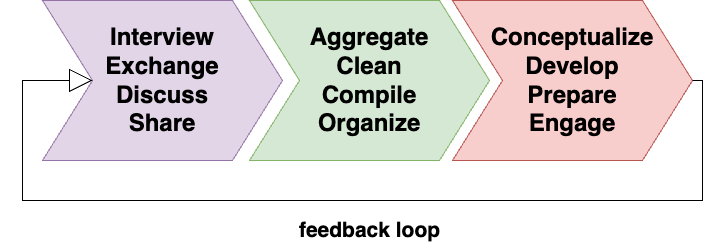
\includegraphics[width=1\linewidth]{Modele_Latex_CNRIUT2025//images/Diagrams-Simplified framework chain Our approach.drawio.png}
    \caption{Chaîne d'approche simplifiée}
    \label{fig:approach-simplified}
\end{figure}

La première phase (en violet) de discussion est primordiale et, peut-être, la plus longue et la plus importante étape dans notre cadre. Pour que le système soit fiable, efficace et accepté, vous devez faire sentir à tous les acteurs impliqués qu'ils sont écoutés et qu'ils sont intéressés par le système. En prouvant que c'est un outil vital pour eux et l'alliance et que suivre un tel cadre est important pour le bien-être de l'alliance et de toutes les actions (y compris les leurs).

La deuxième phase (en vert) évalue les résultats de la première étape. Comment pouvons-nous agglomérer et compiler les informations de la première phase pour qu'elles soient à la fois logiques et pertinentes pour tous ? C'est là que les experts et les chefs de projet devront discuter et échanger sur la meilleure façon de compiler toutes les données acquises à partir de la phase 1 pour développer la solution.

Enfin, la troisième phase, en rouge, est la conception, le développement et la construction du système de suivi et d'évaluation concret. Représenté comme un entrepôt de données pour l'impact et une plateforme de partage de connaissances et de collaboration opérée à travers les technologies sémantiques et les technologies du web sémantique.

Chaque étape inclut des plans pour évaluer le changement à l'intérieur de l'université et de l'alliance dans son ensemble. À travers la planification informative et les actions de suivi pour gérer la résistance et simplement guider le changement à travers l'alliance, pour qu'il soit perçu positivement. Il est clair, à partir de la revue de la littérature, que pour avoir un changement efficace, nous devons créer une boucle de rétroaction positive pour nous assurer que tous les acteurs impliqués dans l'action se sentent écoutés et entendus. 